\documentclass{sigchi}

\usepackage{amsmath}
\usepackage{amssymb}
\usepackage{amsfonts}
\usepackage{bm}
\usepackage{xcolor}
\usepackage{booktabs}
\usepackage{floatrow}
\usepackage{blindtext}
\usepackage[english]{babel}
\usepackage[utf8x]{inputenc}
\usepackage[colorinlistoftodos]{todonotes}
\usepackage{graphicx}
\usepackage{tabularx}

% \long\def\/*#1*/{}

% https://www.overleaf.com/5725947pwvcgh#/18690373/

%Achievement, Relationship, and Engagement (ARE): Using 
% 
\title{Deep Reinforcement Learning for Modeling User Strategies and Motivations from Massive Game Behavioral Data}

\numberofauthors{4}
\author{%
  \alignauthor{Leave Authors Anonymous\\
    \affaddr{for Submission}\\
    \affaddr{City, Country}\\
    \email{e-mail address}}\\
  \alignauthor{Leave Authors Anonymous\\
    \affaddr{for Submission}\\
    \affaddr{City, Country}\\
    \email{e-mail address}}\\
  \alignauthor{Leave Authors Anonymous\\
    \affaddr{for Submission}\\
    \affaddr{City, Country}\\
    \email{e-mail address}}\\
  \alignauthor{Leave Authors Anonymous\\
    \affaddr{for Submission}\\
    \affaddr{City, Country}\\
    \email{e-mail address}}\\
}


\begin{document}
\maketitle

\abstract


Game user research, which investigates interactions between players and games, is one of the most popular topics in HCI field. However, previous studies are mostly exploratory and descriptive, failing to capture the richness and complexity of game user behaviors. Inspired by recent success of reinforcement learning (RL) algorithm in game strategies, we present a novel RL method to model the underlying motivations which induces the user behaviors we observed. It further reveals the playing strategies which is used to predict user behaviors. We use a massive and complex online game behavioral dataset, World of Warcraft Avatar History (WoWAH), which records over 70,000 users' log data spanning 3 years time period. Our model not only can predict users' behaviors with a high level of accuracy. Moreover, it can also reveal users' motivation dynamics, in terms of \textit{achievement}, \textit{social}, and \textit{immersion}.
%Massively multiplayer online role-playing game (MMORPG), such as World of Warcraft (WoW), attracts millions of users and many of them spend thousands of hours playing games online.
%Understanding their behaviors and the underlying motivations is of great interests to game designers and researchers, and also to parents and educators.
%We employ deep reinforcement learning algorithm to model users' playing strategies, and propose an inverse reinforcement learning algorithm to model their motivations.
%We use a massive and complex online game behavioral dataset, World of Warcraft Avatar History (WoWAH), which records over 70,000 users' log data spanning 3 years time period.
%Our trained model not only can predict users' behaviors with a high level of accuracy.
%Moreover, it can also reveal users' motivation dynamics in terms of \textit{achievement}, \textit{social}, and \textit{immersion}.

\category{H.5.m}{Information Interfaces and Presentation (e.g. HCI)}{Miscellaneous} \category{I.2.1}{Artificial Intelligence}{Applications and Expert Systems}
\keywords{Online game motivation; game design; reinforcement learning; apprenticeship learning;}

\section{Introduction}

Understanding Massively multiplayer online role-playing game (MMORPG) games satisfaction mechanism and user behaviors could be non-trivial.
As human players have a mixed feeling from different perceptions and they act not for a concrete, explicit objective such as winning an episode or taking high scores.
While it's plausible to build a gaming bot from the player log data, to advance in the game, it ignores other dimensions of motivation which the players also care about.
The game designers and researchers, also parents and educators, are, however, keen to reveal the underlying mechanism instead of just mastering the game.

\begin{table}[t]
    \centering
    \caption{WoWAH Dataset Attributes}
    \begin{tabularx}{\textwidth}{lX}
        Attribute & Value \\
        \midrule
        Duration & 1107 days \\
        Sample Interval & Every 10 minutes \\
        \#Users & 70,000+ \\
        Locations & One of 165 zones
        \label{tbl:wowah}
    \end{tabularx}
\end{table}

Take World of Warcraft (WoW), which is one of the most successful MMO games in the world, as an example.
It's massive, and multiplayer as millions of players pay to subscribe the game platform.
On the platform players can communicate with others, finish some quests cooperatively, compete with each other, and even build their own guilds.
WoW also provides different kinds of races, careers and optional requests that could serve players with extra flexibility to evolve different game styles.
With all those features the players' behavior can be very complex, as they receive different dimensions of satisfaction which eventually compose the general reward system of the game.
%With all those features the players receive many different dimensions of satisfaction which eventually compose the general reward system of the game.
%It was released by Blizzard in 2004 and stills continuing updating nowadays.

For its huge research and commercial value to study game players' behavior, attentions has been drawn for both qualitative and quantitative studies.
In contrary to WoW, many studies are conducted on single-player game or multi-player but zero-sum game.
For those environments, advancing usually serves as the sole criterion of game motivation.
In Game Trace Archive (GTA) \cite{guo2012game} who has been collecting online gaming data since 2012, 10 out of 14 traces are from the game environment stated above.
Although reinforcement learning (RL) algorithms have been succeeded in mastering such kind of games, it does not help figuring out the underlying motivation, neither the complex reward mechanism existing in MMO games and in real world.
Even for those studies in WoW, datasets such as Very Large WoW Armory Dataset \cite{Bell2013a} focus on certain campaigns instead of general gaming strategies because of its short time span and fine-grained actions (such as spelling).
Taking that into consideration, the episodes recorded is still mostly about advancing, and game tactics.

World of Warcraft Avatar History (WoWAH) dataset \cite{lee2011world}, published in 2011, records the location (in term of zone) of over 70,000 users every 10 minutes, together with some essential statistical analysis.
%\footnote{we talk about the reason choosing this dataset in the first section of \textit{Method}} 
However, those analysis and the further studies based on the dataset are far from fully utilization of the data.
While some of them use simple classifiers or clustering for behavior analysis \cite{suznjevic2011mmorpg,drachen2014comparison}, others focus on forecasting future events such as unsubscribing of game or violation of terms \cite{bauckhage2015clustering,thawonmas2011analysis,lou2012forecasting}.
Few of them are effectively modeling the interaction between the players and the game environment, neither on another dataset. 
On the other hand some studies tries to conduct studies on player motivations \cite{Bell2013a}, but only able to apply some basic machine learning tools such as clustering.
%First, statistical approaches usually collapse the data over the time scale, which ignores the dynamic of both gaming environment and players.

We re-employ the WoWAH dataset in a totally different way: to model human-computer interaction (HCI) from a reinforcement learning perspective.
The human player and computer are characterized by a pair of agent and environment, as shown in Fig. \ref{fig:chi}.
We show an interesting analogy between the traditional user experience model on the left, and the reinforcement learning scheme on the right.
In the model, each player is modeled by an agent, whose zone transactions are regarded as the actions of the agent.
Instead of manually collect opinions from the players as the feedback, we utilize the actual reward system of the game which provide diverse satisfactions.
A common difficulty in WoW and most of the cases in HCI is that the definition of reward is implicit or partial, e.g. we can't tell if a play is optimal simply by looking at the experience gain credited to this play.
Even if some could try building a reward function according to their knowledge of certain environments, it worth to note that figuring out the reward mechanism itself is a valuable task.
In fact, the, usually underlying, reward mechanism gives the most succinct description of the task.
Especially for the developers of the environment, it's a way to give a quantitative representation of what they have designed.
%Existing models in reinforcement learning succeed in modeling human behaviors by training the agent to maximize the explicitly defined reward.

\begin{figure}[t]
    \centering
    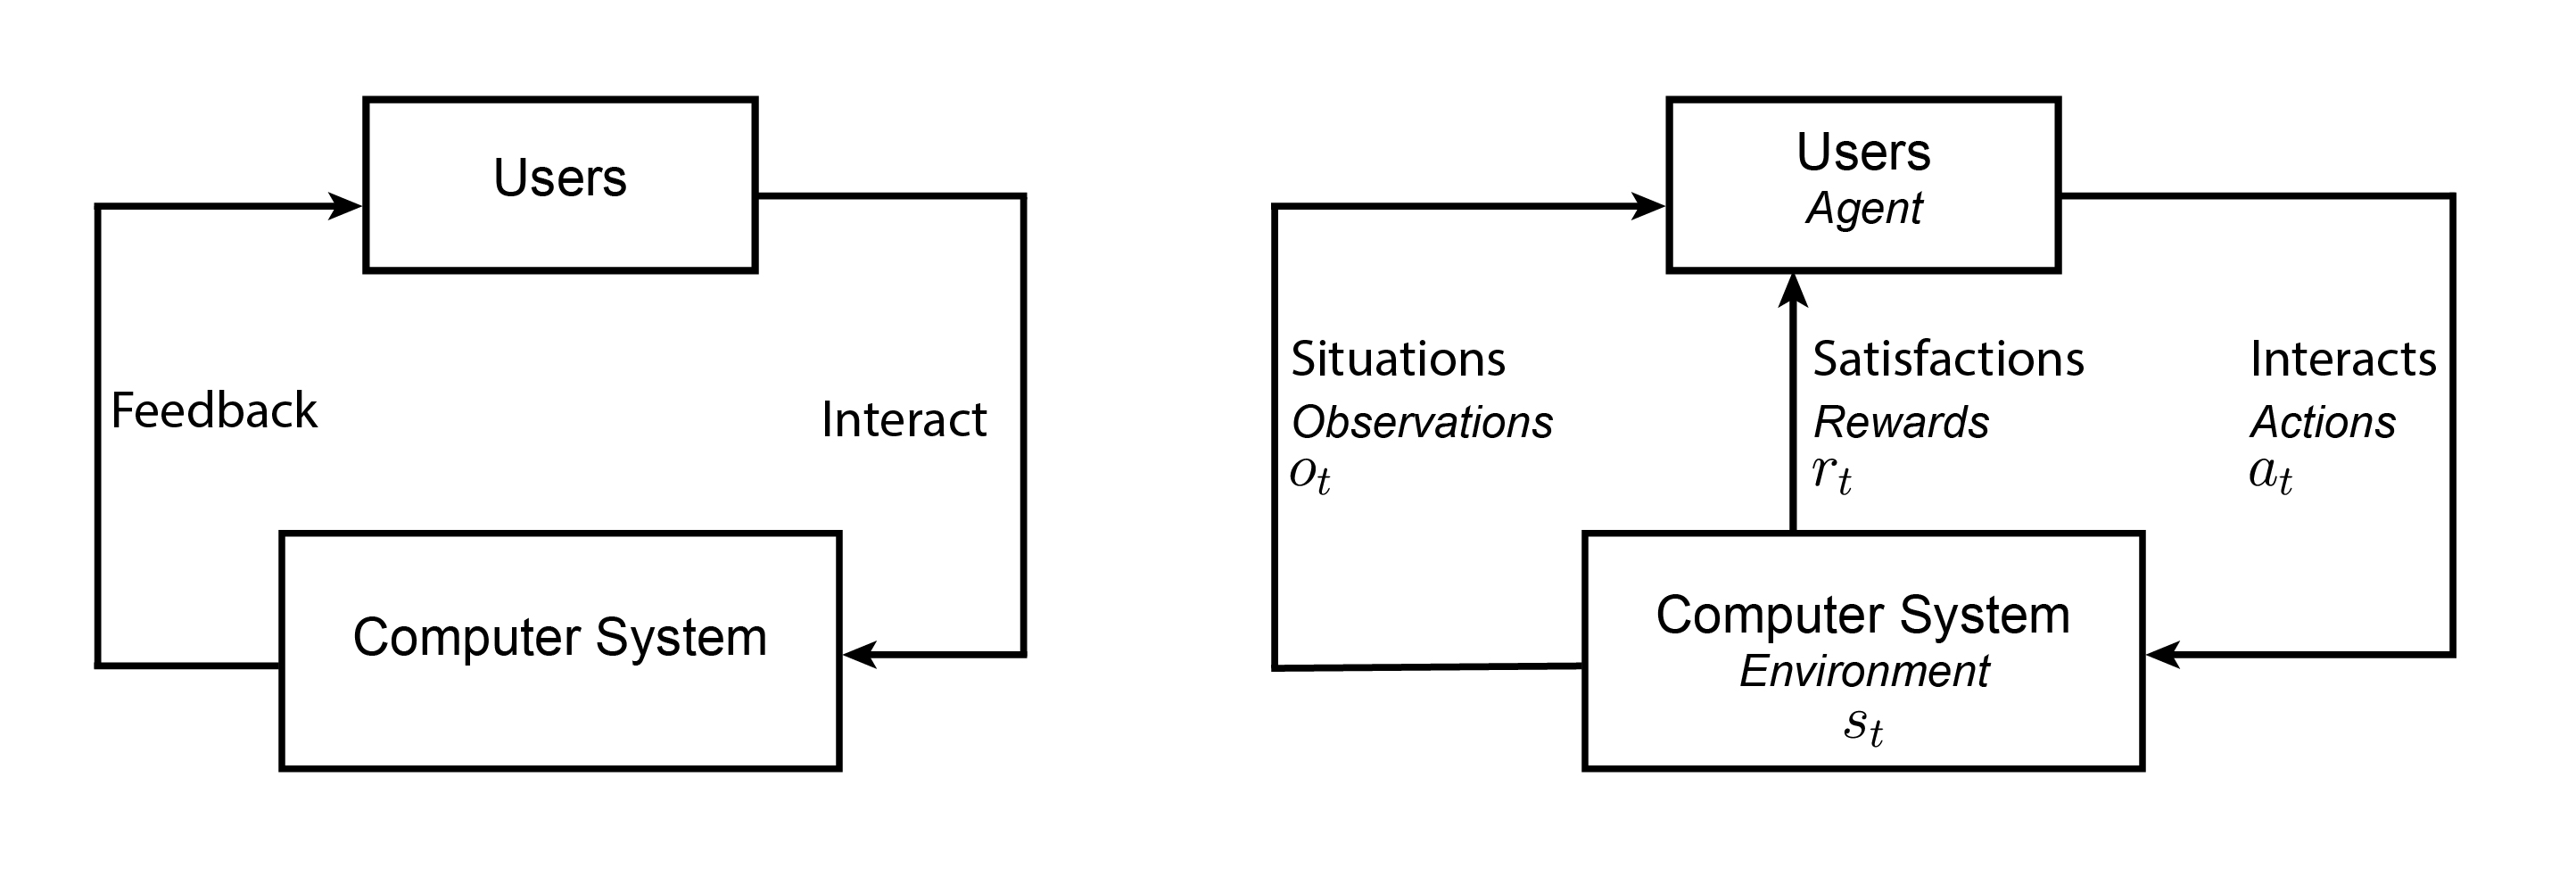
\includegraphics[width=\textwidth]{figs/rl-vs-chi.jpg}
    \caption{User experience model (left) and reinforcement learning model (right)}
    \label{fig:chi}
\end{figure}

The process of recovering the reward function is inverse reinforcement learning (IRL).
In a data-driven manner, it recovers the underlying reward function which induces the recorded user behaviors, simply by assuming that those players are trying to maximize their rewards.
Most of the IRL algorithms require we have access the dynamic of the environment, that is in WoW, we simulate the player's action and observe the feedback from the environment.
Although we obviously don't have it, we address it by proposing an IRL algorithm based on purely off-policy learning.
The model analyzes the behaviors of the players, using the trajectories composed of player locations, and returns the reward function under which those trajectories are most plausible to happen.
With the recovered reward, we train an agent to best mimic the general user behavior in WoWAH dataset.
As our reward recovery algorithm works for any set of trajectories, we conduct future studies to character the dynamics of the game environment thus how design factors working on user behaviors, and compare different groups of users to examine the divergence of game motivations.
Consistency was observed between our model results and empirical analysis on the game environment.


\section{Related Work}

\subsection{Online Game Player Motivation And Rewards}

One reason that online games appeal so many players is that it provides the possibility for different kinds of play styles. 
The same online game may have respective meanings for different players.
In the game environment, players pursue certain kinds of satisfactions they want by conducting their actions, which eventually compose the user behaviors we observe.
Hence, it's natural to assume a user's behaviors are highly correlated with the user's specific reward mechanism, represented by their demanding satisfactions.
And for game designers and research, finding the demanding satisfactions of users could yield better understanding of the game, and ease to serve the users with better experience.

Previous study categories the satisfactions into three major aspects, namely, achievement satisfactions, social satisfactions, and immersion satisfactions \cite{yee2006motivations}.
It was then divided into ten subcategories, briefed in Table. \ref{tbl:components}.
More details are provided in the original paper and the author's another paper about MMORPG motivation \cite{yee2006demographics}.
The satisfaction model is popular in online game researches, and provide some basic understand of the online game motivation.
However, the weights associated with these ten kinds of satisfactions are still unknown.
As the weights basically depicts a user's profile, it would be very meaningful if they can be recovered in a purely data-driven process, i.e. based on the user's playing history.

\begin{table}
\caption{Components of game motivation}
\begin{tabularx}{\textwidth}{lX}
    Components & Sub-components \\
    \midrule
    Achievement & Advancement, Mechanics, Competition \\
    Social & Socializing, Relationship, Teamwork \\
    Immersion & Discovery, Role Playing, Customization, Escapism
    \label{tbl:components}
\end{tabularx}
\end{table}

\subsection{Player Behavior Analysis in Online Games}

In game user research, several methods used to evaluate playability and usability of games.
Namely, \textit{Think Aloud Protocol}, \textit{Retrospective Testing}, \textit{Heuristic Evaluation} \cite{pinelle2008heuristic} and \textit{Physiology-based Playtesting} \cite{mirza2011understanding} are four qualitative research methods \cite{desurvire2013methods}.
Those methods provide fast and efficiency results, however, it cannot learn all users' motivations in the games \cite{kivikangas2011review}. 
Moreover, it is difficult for researchers to evaluate the results based on the qualitative psychology model. 
For instance, \textit{Heuristic Evaluation} is the method used in small expert player group and it only gets result from expert feedback, while in large game different motivations are driven by different kinds of users. 
Thus it is not possible to use it to model common users' ideas \cite{desurvire2013methods}.

Despite those qualitative user research methods, \textit{Frequency Data Analysis} \cite{el2013game}, \textit{A/B Testing} \cite{lange2009initial} and \textit{Experimental Factorial Design} \cite{ebner2007successful} are the most common quantitative user testing methods.
\textit{Frequency Data Analysis}, which was previously used in WoWAH dataset \cite{Bell2013a}, is mostly based on factorial type and time series statistic method. 
It can only evaluate single variables in the model, while for some complex games, the players behaviors and motivations are not unary. 
The motivations are multiple and even mixed in a real game environment. 
Those restricts leads to difficulties for researchers to use linear handcraft model to formulate user behaviors. 
In order to get better understand about multi-users' behavior model, more complex and powerful model, such as reinforcement learning, are needed for game user research.

\subsection{Reinforcement Learning and Inverse Reinforcement learning}

Reinforcement learning (RL), especially deep reinforcement learning (DRL), is an emerging domain inspired by behaviorist psychology. 
In RL, the agent performs in an online environment and conducts a sequence of actions.
Instead of being taught of the correct policy, the agent get a reward for each of its actions and evolves itself from its own pains and pleasures.
Interestingly, it deals with the common trade-off between exploration and exploitation, which presents in many real life situations.
Success in maximizing cumulative reward in the future, rather than exploiting current reward, could lead to expert level game play, which is also a intrinsic property of expert human players.
For example, to level up quickly in a game in a long-term perspective, the player has to conduct some preparation works which does not necessarily benefit its leveling up in the near future.

RL is able to formulate many problems in user behaviors analysis and modeling.
For example, the recent advances in RL conduct superior play compared with professional human players in the game of Go \cite{silver2016mastering}, Atari 2600 \cite{mnih2015human}, and Poker \cite{heinrich2016deep}.
It's also employed to model users' clicking and browsing behaviors for online shopping websites, and robotics and optimal controls.
It's worth to note that DRL makes it possible to handle complex environment with high-dimension observation spaces, making it possible to model a wide range of problems such as WoW user behavior analysis.

A great challenge is that the reward scheme of the environment is not explicitly given in most problems in user behavior analysis and modeling.
For example, the user experience of a software or an online game is the combination of different kinds of satisfaction, processed by the human brains.
In some of those cases, inverse reinforcement learning (IRL) \cite{ratliff2006maximum,ng2000algorithms} recovers the underlying reward function, using the recorded actions of the users.
Further applying apprenticeship learning algorithms \cite{abbeel2004apprenticeship} could mimic the policy that was used to generated the recorded data.
But to invoke those IRL algorithms, it usually requires the access of the dynamic of the environment, which is not doable in online gaming analysis.
As applying IRL on users' behavior log could help the developers understand the intention of the user, New IRL algorithms are needed to be designed to comply with the problem without the access to the dynamics.

\section{Method}

\subsection{Dataset Description and Reinforcement Learning Formulation}

We use World of Warcraft Avatar History (WoWAH) dataset \cite{lee2011world}, collected from realm \textit{TW-Light's Hope} during 1st Jan 2006 to 10th Jan 2009.
It contains 70,055 users after we filtering out those with too short playing history, each with 516.21 time intervals (5162.1 minutes) spent online on average.
During each of the 10-minute interval, the user's location, in terms of zone ID (ranging from 1 to 165), was recorded.
The players' trajectories was composed of a sequence of locations, which reflect their playing strategies.
We find datasets with coarse-grain records, i.e. 10-minute interval, most suitable to model user behaviors.
They are preferred than those with interval of a few seconds, which instead focus on game tactics and user mobility \cite{Bell2013a,shen2014characterization}.
Moreover, the dataset contains many different kinds of users: both novice and expert, guild members and isolated players, low-level and high-level players etc. with their respect class, and race in game.
The detailed attributes are listed in Table~ref{tbl:wowah}.

In a reinforcement learning perspective, we treat an user as the agent who conduct an action every time interval.
An action here corresponds to a zone transaction or staying in the current zone.
The user receives current stats of its profile as the observation, after each action it has conducted.
The observation includes all the attributes recorded in the dataset, cached by a certain number of time intervals, after a pre-processing to reduce the redundancy.
To make the data consistent, we ignore the time intervals where a user being offline, and concatenate multiple game session of a player to build the trajectory.
As the exact reward mechanism remains unknown, the RL policy can only be learned after the reward function is properly modeled.

We process some preparation for the reward modeling.
Borrowing the result in game motivation analysis \cite{yee2006motivations}, we define and compute different of satisfactions using the WoWAH dataset.
The constructions of $f_1,\dots, f_5$ are illustrated in Table \ref{tbl:satisfactions}, which are able to be calculated from the observations the user receives.
With those value, we assume the reward function which the agent tries to optimize during the game play, is associated with the five different dimensions of satisfactions.
We further address the relation between the reward function, and the satisfactions.
Note the value of $f_1,\dots, f_5$ are normalized into the same scale.

\begin{table}
\caption{Different types of satisfactions (Sat.), and their corresponding categories}
%\begin{tabular}{llp{4.8cm}}
\begin{tabularx}{\textwidth}{lX}
    Sat. & \textbf{Category} \& Definition \\
    \midrule
    $f^1$ & \textbf{Advancement} The speed the user collecting experience and leveling up in game. It's the most common satisfaction a user could receive. \\
    $f^2$ & \textbf{Competition} The satisfaction the user get by joining battleground or arena and competing with human opponents. \\
    $f^3$ & \textbf{Relationship} The long-term relationship with the user's guild, which is quantified by the time elapse since the user joining its guild. \\
    $f^4$ & \textbf{Teamwork} The satisfaction the user get by playing in a zone which is featured by teamwork, e.g. \textit{Battleground}, \textit{Arena}, \textit{Dungeon}, \textit{Raid}, or a zone controlled by \textit{The Alliance}. \\
    $f^5$ & \textbf{Escapism} Escapism begins to accumulate if the user has been online for a long session or has been regularly login to the game for many days.
    \label{tbl:satisfactions}
\end{tabularx}
\end{table}

\subsection{Reward Mechanism Modeling}

We present our algorithm to recover the underlying reward mechanism of the players, using the trajectory $\tau$ of a user or a group of users.
Assume the reward a user receives is the convex combination of the five kinds of satisfactions listed in Table. \ref{tbl:satisfactions}.
Let $f_t=(f_t^1,f_t^2,f_t^3,f_t^4,f_t^5)$ be the vector of satisfactions the user received at time $t$, we have the total reward the user receives at time $t$
\begin{equation*}
r_t=\phi^Tf_t,
\end{equation*}
where $\phi$ is the combination weight with $||\phi||_1=1, \; \phi \geq 0$.
Assume at each time step, the user tries to take an action $a$ according to the current game state $s$ so as to maximize the best expected cumulative discounted (with discount $\gamma$ over time) reward $Q^\ast(s, a)$, where
$$Q^\ast(s,a)=\mathbf{E}[R_t | s_{t}=s, a_{t}=a | \pi^\ast]$$
and
$$R_t=\sum_{t^\prime\geq t}\gamma^{t^\prime-t}r_{t^\prime}=\sum_{t^\prime\geq t}\gamma^{t^\prime-t}\phi^Tf_{t^\prime}.$$
The term $\pi^\ast$ indicates optimal policy, described by a probabilistic distribution $\mathbb{P}(a|s)$ over the feasible action space $\mathcal{A}(s)$, and $Q^\ast$ is also known as the action-value function.
In this setting, the weight $\phi$ must satisfy that the action the user has taken must induce a larger $Q^\ast$ value than any other valid action would have done.
This optimality infers that
\begin{equation}
Q^\ast(s,a) \geq \max_{a^\prime \in A(s)}Q^\ast(s,a^\prime)
\label{eqn:irl}
\end{equation}
is satisfied for all $(s,a)$ pairs appeared in the user's trajectory.
Consider the existence of possible sub-optimal actions, we introduce slack variables $\xi_{s,a}$ into the Eq. \eqref{eqn:irl} to make it feasible.
Let $\xi_{s,a}$ be the difference of the actual action-value $Q^\ast(s,a)$, and the largest possible action-value $\max_{a^\prime \in A(s)}Q^\ast(s,a^\prime)$ whenever Eq. \eqref{eqn:irl} is not satisfied, and zero otherwise.
We minimize the summation of $\xi_{s,a}$ over the recorded user's trajectory
\begin{equation}
-C\sum_{s,a} \left[\min(0, Q^\ast(s,a) - \max_{a^\prime \in A(s)\backslash a}Q^\ast(s,a^\prime))\right], \label{eqn:slack}
\end{equation}
which is then formulated into the following linear programming (LP) problem

\begin{equation}
\begin{aligned}
& \underset{\phi, \xi}{\mathrm{minimize}}
& & C\sum \xi_{s,a} \\
& \mathrm{subject}\text{ }\mathrm{to}
& & \phi^T(\tilde{Q}(s,a)-\tilde{Q}(s,a^\prime)) \geq - \xi_{s,a}, \\
&&& \quad\quad\quad \forall (s,a) \in \tau, a^\prime \in \mathcal{A}(s)\backslash a \\
&&& \phi \geq 0, \; ||\phi||_1\geq 1\\
&&& \xi_{s,a} \geq 0, \; \forall (s,a) \in \tau. 
\label{eqn:lp}
\end{aligned}
\end{equation}
In formula \eqref{eqn:lp}, $\tilde{Q}(s,a)=(Q^1,Q^2,Q^3,Q^4,Q^5)^T$, and
\begin{equation}
Q^i(s,a)=\mathbf{E}[\sum_{t^\prime\geq t}\gamma^{t^\prime-t}f^i_{t^\prime} | s_{t}=s, a_{t}=a | \pi^{i,\ast}] \label{eqn:qi}
\end{equation}
is the action-value function, when the user only takes the $r=f^i$ into account and ignores all 4 other kinds of satisfactions.
The LP formulated above is equivalent to minimizing Eq. \eqref{eqn:slack} because by definition we have $Q^*(s,a)=\phi^T\tilde{Q}(s,a)$

\begin{figure*}[t]
  \centering
  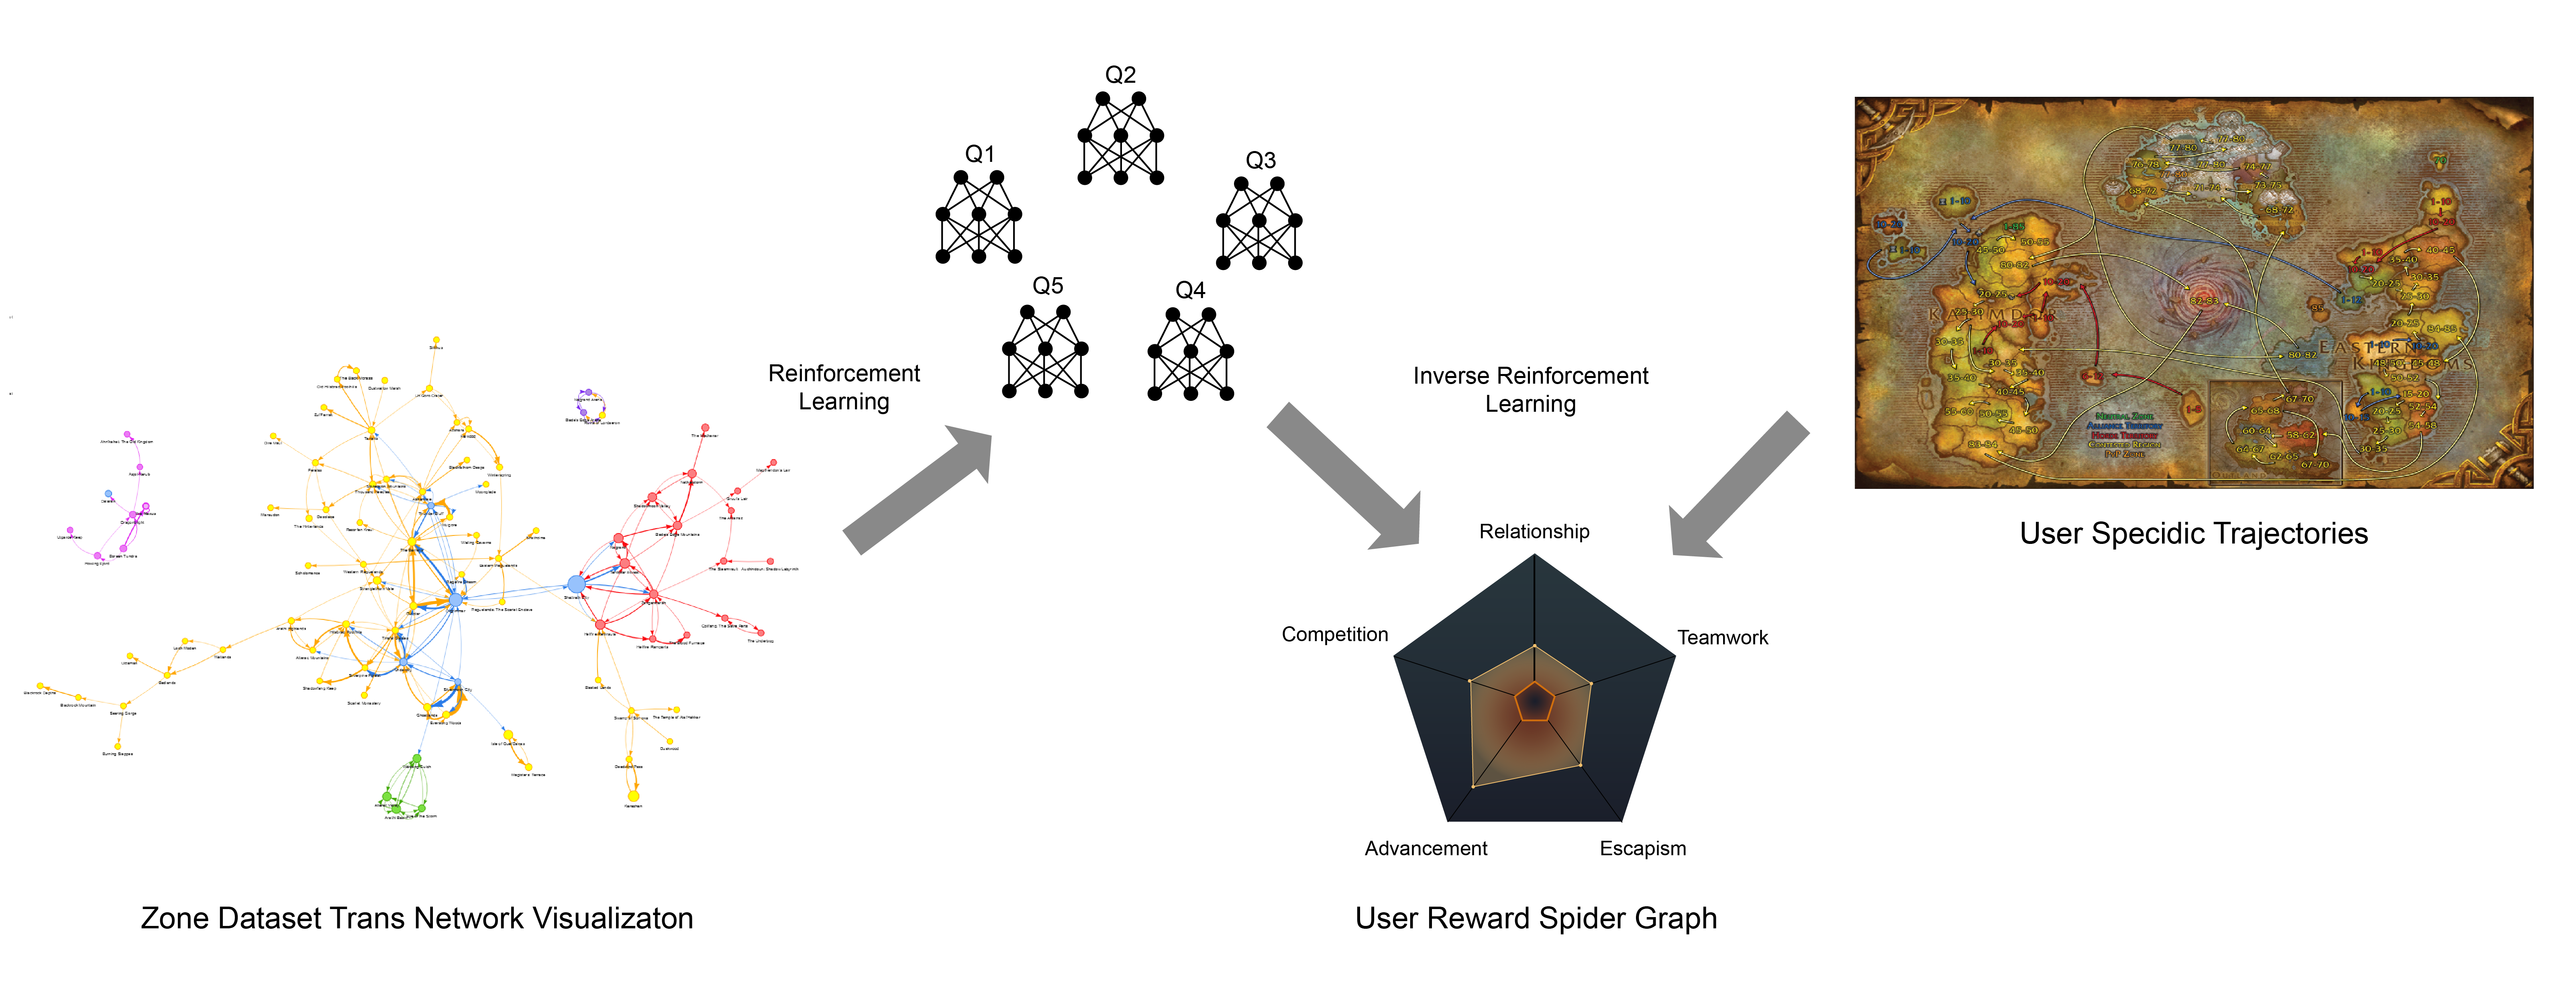
\includegraphics[width=\textwidth]{figs/workflow.png}
  \caption{Workflow to recovery the underlying reward mechanism using RL and IRL.}
  \label{fig:workflow}
\end{figure*}

\subsection{Action-Value Function Approximation}

As LP can be solved efficiently, it suffices to estimate $Q^i(s,a)$.
As the number of possible states $s$ could be arbitrary large for an user in WoW, it's impossible to enumerate over the state space as typical Markov Decision Process (MDP) does.
Instead, we build deep-Q networks (DQN) \cite{mnih2015human} to approximate the $Q^i$ functions.
The network takes the observation as input which is used to represent the state $s$, and output the $Q$ value for every action $a$.
Taking advantage of the fact that DQN is a general framework for multiple environments, we use the same network architecture for $i=1,\dots,5$ as illustrated in Fig. \ref{fig:architecture}. 
The categorical elements in $s$ are firstly processed by an embedding layer \cite{mikolov2013distributed}, while the numeral elements are fed into an fully connected (FC) layer with rectifier non-linearity. 
The output of embedding layer and FC layer are then concatenated and fed into another FC layer with rectifier non-linearity. 
A final FC layer is applied to compute the $Q(s,a)$ value for each action $a\in\cup_s\mathcal{A}(s)$.

Denote the trainable parameters in the Q-network as $\theta^i$, we optimize over $\theta^i$ in order to approximate Eq. \eqref{eqn:qi}.
The key observation of Q-learning is that, the action-value function, by its definition, should satisfy the Bellman equation.
That is, if the user takes action $a$ and the state turns into $s_{t+1}$ from $s_t$, we have (recall $f_t^i$ is the reward associated with $Q^i$)
\begin{equation}
Q^i(s_t,a_t)=f_t^i + \gamma \max_{a^\prime}Q^i(s_{t+1}, a^\prime). \label{eqn:bellman}
\end{equation}
Q-learning tries to find the action-value function satisfying Eq. \eqref{eqn:bellman}, by minimizing the squared difference $L$ between both sides of the Bellman equation
\begin{equation*}
L^i=\mathbb{E}_{s_t, a_t, f_t^i, s_{t+1}} \frac{1}{2}(Q^i(s_t,a_t)- f_t^i - \gamma\max_{a^\prime}Q(s_{t+1}, a^\prime))^2.
\end{equation*}
Since $L^i$ is differentiable with respect to $\theta^i$, $\theta^i$ can be updated via stochastic gradient descent, by
\begin{eqnarray}
\theta^i \leftarrow \theta^i - \alpha\frac{\partial L}{\partial \theta^i}\Big|_{s_t, a_t, f_t^i, s_{t+1}}
\label{eqn:sgd}
\end{eqnarray}
Different from the algorithm introduced in \cite{mnih2015human}, that the target network $Q(s_{t+1}, a^\prime)$ only get updated periodically, we put vanilla different of $L^i$. 
This is because when using log data, we can easily sample from the dataset randomly and the instability of DQN caused by the correlation between consecutive frames can be avoided.
The derivative of $L$ with respective $\theta^i$ is then
\begin{equation*}
\begin{aligned}
\frac{\partial L}{\partial \theta^i} = & \mathbb{E}\Big[ (Q^i(s_t,a_t)- f_t^i - \gamma\max_{a^\prime}Q(s_{t+1}, a^\prime)) \\
& \cdot (\frac{\partial{Q^i(s,a)}}{\partial{\theta^i}}|_{s_t,a_t} - \frac{\partial{Q^i(s,a)}}{\partial{\theta^i}}|_{{s_{t+1},a^\ast}})\Big],
\end{aligned}
\end{equation*}

where $a^\ast$ is the action which maximizes $Q^i(s_{t+1},a)$.

\begin{figure*}[t]
  \centering
  \includegraphics[width=\textwidth]{figs/architecture.png}
  \caption{DQN architecture for $Q^i$ training, $i=1, \dots,5$}
  \label{fig:architecture}
\end{figure*}

\subsection{Policy and User Behaviors}

Solving LP \eqref{eqn:lp}, the action-value function $Q^\ast(s,a)$ over the underlying mechanism is known for the user/users who conducted trajectories $\tau$.
As assumed by the definition of $Q^\ast(s,a)$, player pursuing cumulative reward $R_t$ should follow the action $a^\prime$ which leads to largest $Q^\ast(s,a^\prime)$.
Which induces the policy
\begin{equation}
\pi^\ast(s) = \text{argmax}_{a^\prime}Q^\ast(s,a^\prime).
\label{eqn:policy}
\end{equation}
Although $\pi^\ast(s)$ may not be the one who advances fastest in game (which should instead be $\pi^1(s) = \text{argmax}_{a^\prime}Q^1(s,a^\prime)$), it is able to mimic the actions that in general a player would conduct. 
That is, the policy $\pi^\ast(s)$ can be used to predict the action of users, even when they are under mixed and complex reward mechanism.

Using similar idea, during the training of $Q^1$ network, we evaluate the quality of the Q-learning process.
Consider collecting experience and getting level up is one of the major objective for players, we examine if the actions predicted by $Q^1$ agree with the moves conducted by those who level up quickly. 
For the $(s,a)$ pairs extracted from the top 200 (in term of leveling up speed) players' trajectories, we try to find if $a$ matches $\pi^1(s)$. 
The prediction accuracy is 0.49 which is decent considering the total number of feasible actions $|\cup_s\mathcal{A}(s)|=165$, corresponding to 165 different zones in WoW existed during Jan 2006 - Jan 2009. 
It's competitive with 0.53, using behavioral cloning \cite{amit2002parametric,sammut1992learning} with classifier, and outperforms 0.23 if we approximate the $Q$ function using linear function. 
Note that we are not intended to benchmark the accuracy.
Instead we use these quantitative evaluations to ensure that the optimization \ref{eqn:sgd} well converges and produces meaningful action-value approximation.

\section{Results}

Different from previous results about RL prevailing on Atari games \cite{mnih2015human} and zero-sum games \cite{silver2016mastering,heinrich2016deep}, our approach models the user motivation and behavior instead of simply pursuing advancement. 
Using Table. \ref{tbl:satisfactions} and solve LP \eqref{eqn:lp} on a trajectory pieces randomly drawn from the original WoWAH dataset, the universal underlying reward mechanism of the player community is revealed as $\phi=(0.61, 0.16, 0.07, 0.05, 0.10)^T$. 
In another words, when conducting a behavior, the user's consideration is composed of 61\% there advancement, 16\% their competition, 7\% their relationship, 5\% their teamwork, and 10\% their escapism on average. 
The results is illustrated as a spider map in Fig. \ref{fig:spider}.
While game designers, researchers, and parents and educators are meticulous with the motivation of play, we provide an scientific and quantitative way to demonstrate it.

Armed with our model we conduct three different kinds further studies on WoW user research, sketch in the workflow graph in Fig. \ref{fig:results}.
First we show that our model better describes the user behavior, than those who takes only single satisfaction metric.
After modeling the underlying reward mechanism of the environment, we predict the move of the average users, instead of just suggesting the best move for advancing (as $Q^1$ does).
The prediction made by our model is more consistent and accurate than any other trial does.
We then show, using our model, the dynamic of underlying user motivation over time. 
As the motivation system adapts itself over time, WoW adjusts its reward system to make the game more popular.
Especially, observing the dynamics around the release of patch \textit{Wraith of the Lich King}\footnote{http://us.battle.net/wow/en/game/patch-notes/3-0}, it shed some light on how game designs would affect the environment in a quantitative way.
Finally we show the divergence of the underlying reward mechanism between different groups of people. 
One of our analysis matches with the common knowledge, that a player cares more about their \textit{social} than their \textit{achievement} as she/he get more involved into the game.
It make sense to imagine a newcomer spend every minutes collecting experience in order to reach the next plume of golden light for leveling up, meanwhile a veteran sunk in the joy of raiding and chatting with friends.
Since our models is capable to apply to arbitrary group of players as long as they're commonly pursuing any form of reward, it's a powerful tool to categorize and make representation of users, which further benefit techniques such as targeted advertising, targeted recommendation, etc.

\begin{figure}[t]
    \centering
    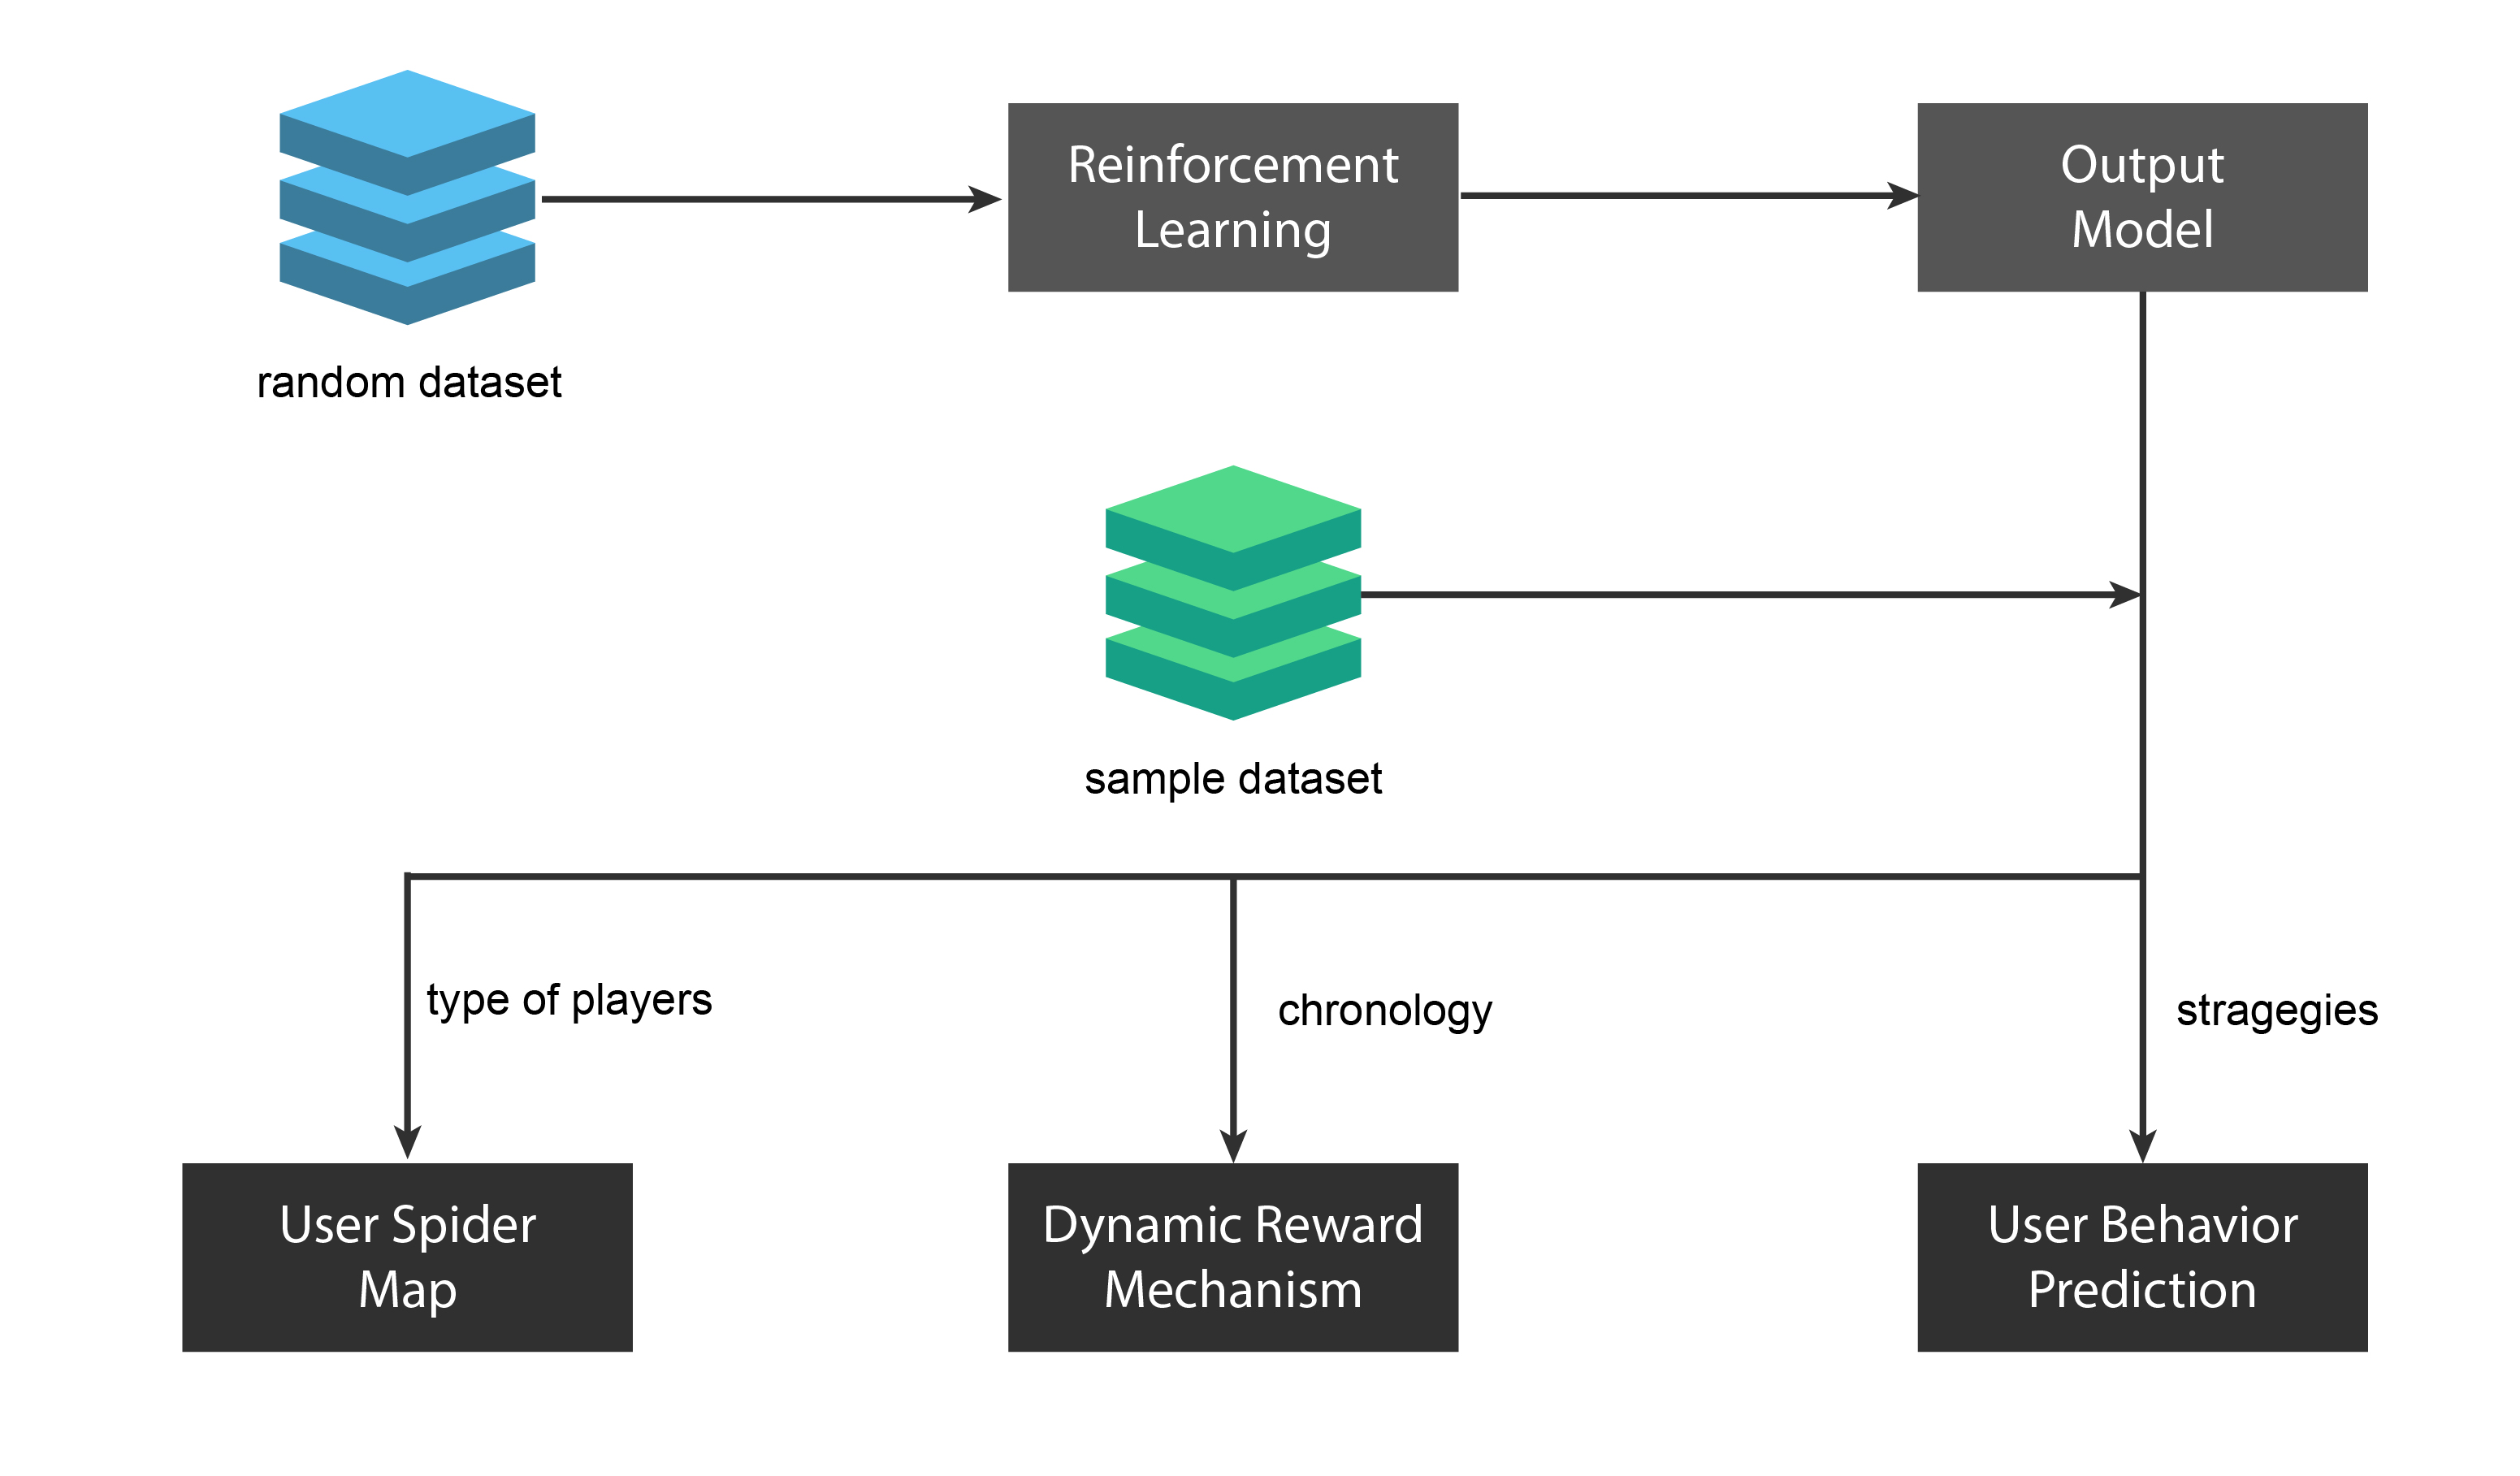
\includegraphics[width=\textwidth]{figs/results.jpg}
    \caption{Workflow to generate our results}
    \label{fig:results}
\end{figure}

\subsection{Predicting User Behaviors}

WoW offers a diverse and complex game environment which serve players with extra flexibility to evolve different game styles.
In RL, to best estimate the general game strategies of a group of users, e.g. those who from have been included in WoWAH dataset, a proper model of reward function is called for rather than a heuristic one.
In fact, any hand-crafted reward function would bias from the actual one, and thus leads to a biased estimation of user behaviors.
In our approach, we firstly solve the SGD \eqref{eqn:sgd} and LP \eqref{eqn:lp} using randomly drown trajectories. 
We then compute the policy using Eq. \eqref{eqn:policy} and compare the output of $\hat{a}=\pi(s)$ with actual action $a$ recorded in the dataset.
We exclude those trajectories that were randomly drown when evaluating the accuracy to keep the integrity, though, it would not have made a significant difference.

We also compare the quality of prediction with behavioral cloning, which straightforwardly learns a mapping from states $s$ to action $a$, using classifiers. 
Two famous successful example were about motor control \cite{amit2002parametric} and fly in virtual environment \cite{sammut1992learning}.
Behavioral cloning usually fails to achieve state-of-the-art result, because the interaction between human and the game was limited by the model assumption of the classifier.
Note that the comparison is for reference only, because we are not trying to just mimic how players moves, but build a model which understand the motivation of those players.
And behavioral cloning by no means could achieve our objective, nor provide any help to understand players or the game (that's also why behavioral cloning not being a popular approach \cite{argall2009survey}).

We show the accuracy of different approaches in Table. \ref{tbl:accuracy}. 
It shows that the accuracy will decrease on average if we apply a disturb on the weight vector $\phi$, making it $\phi+\epsilon$ where $||\epsilon||_1=0, ||\epsilon||_2<<0$ is a disturbance.
It follows the same step in Eq. \eqref{eqn:policy} to acquire the policy.
Also observe from the table that policies induced by single satisfaction factor cannot model user behavior in a high standard.
We also show, by comparing DQN and linear Q-network structure, that the deep architecture illustrated in Fig. \ref{fig:architecture} is necessary to capture the complex and multi-dimensional input.
Finally it occurs that behavioral cloning is competitive with our results.

\begin{table}
\caption{Accuracy of different approaches}
\begin{tabularx}{\textwidth}{ll}
    Approach & Accuracy \\
    \midrule
    $\pi^\ast$ & 56.5\% \\
    Disturbed $\pi^\ast$ & 52.5\% \\
    $\pi^1$ & 45.9\% \\
    $\pi^5$ & 23.2\% \\
    Q-Linear & 29.5\% \\
    Cloning & 55.8\% \\
    \label{tbl:accuracy}
\end{tabularx}
\end{table}

A close look at the errors made in the prediction yields some interesting observations. 
As our models assumes that every players maximizes their cumulative reward in Eq. \eqref{eqn:irl}, the players have been regarded as rational and foresighted.
That is, the players should be able to handle the tradeoff between exploitation and exploration, and not be committed to short-term rewards.
Q-learning achieves this by using cumulative reward as the action-value function, however, humans usually fall into the delayed gratification which has long been recognized \cite{mischel1972cognitive}.
Unfortunately, it would trouble our model which cannot figure if those action are conducted intentionally for some kind of objective or just because of the sub-optimality of play.
Take a pair of users as an example, shown in Fig. \ref{fig:trajectory}.
Both have committed over 3000 hours of play and reached the level 70, the maximum level one can reach at that time.
But the prediction accuracy for the player corresponding to the upper figure (player A) is 67.0\%, compared 39.1\% with the player at bottom (player B).
It's possibly because the fact that our model believes majority of time should not be happened on the same zone the player was spending at the early or middle stage of the game.
But for some player, such as player B, it could be very hard to switch and get out of the familiar place and explore new possibilities for further advancement.
This example would provide a future direction of our work, that to model user behavior, we should not only care about the diverse of motivation, but also the diverse of ability to pursue the reward they want.

\begin{figure}[t]
    \centering
    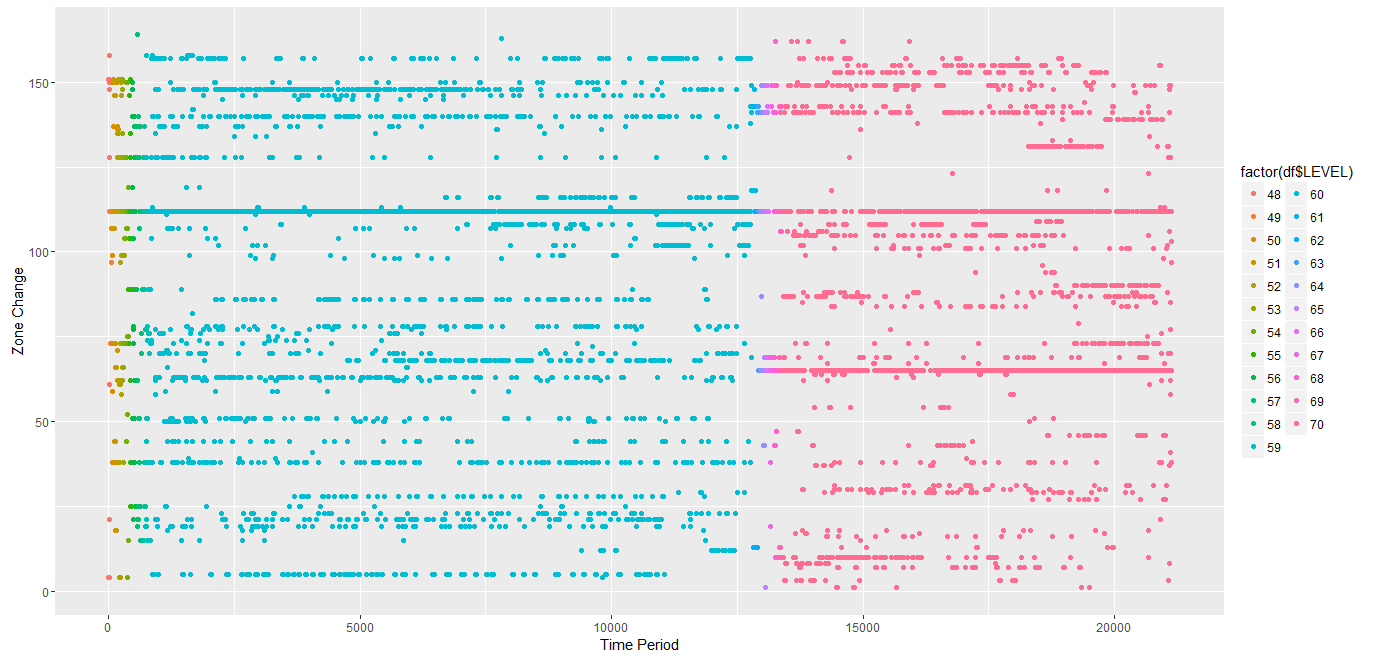
\includegraphics[width=\textwidth]{figs/Rplot31.png}
    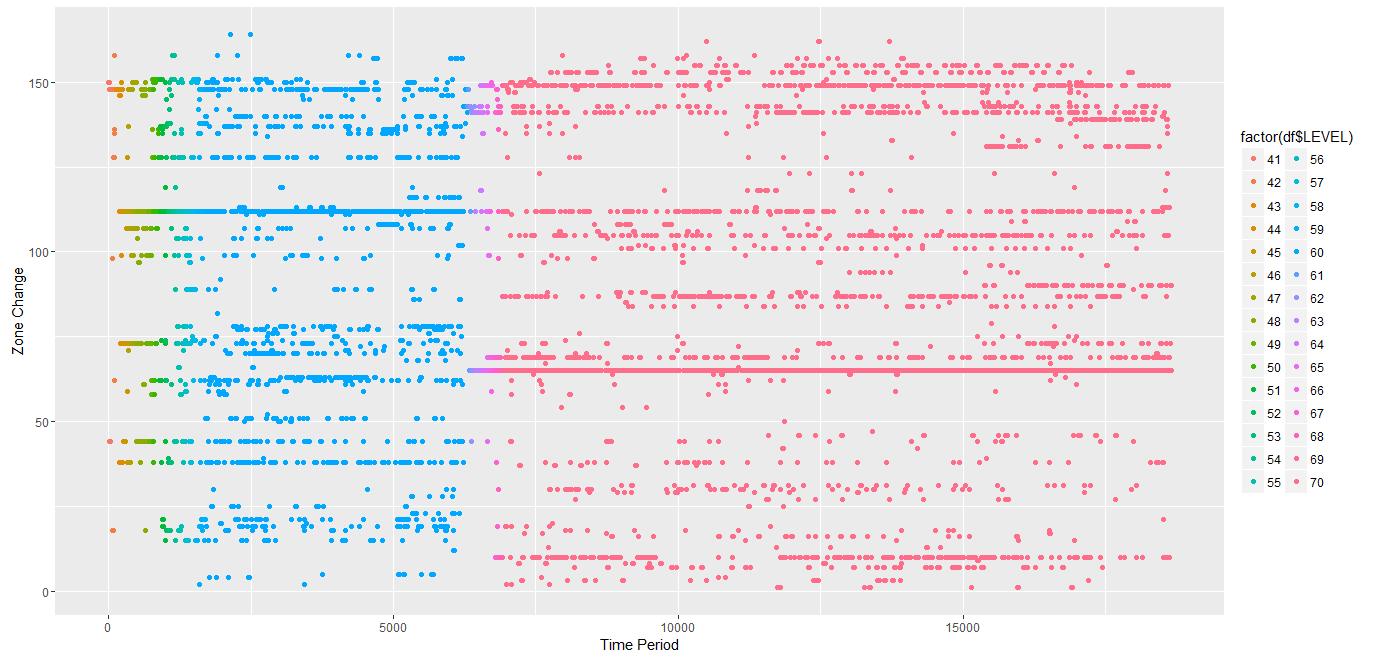
\includegraphics[width=\textwidth]{figs/Rplot36.png}
    \caption{Different Play Styles. The lateral axis indicates play time, with 10 minutes for each time period. and the dot at any time indicate a zone, out of 165 zones, the player was in at that time.. The color of the dots vary as the player levels up.}
    \label{fig:trajectory}
\end{figure}

\subsection{Dynamics of Play Motivation}

The motivation of play could evolve over time, also subject to change as the game gets updated.
Especially, how an update will affect the users' motivation thus users' behavior would be great interest of game designers.
We conduct an analysis on the dynamics of play motivation, i.e. how the underlying reward mechanism changes over time.
The key observation of achieving this is that the set $\tau$ in LP \eqref{eqn:lp} could contain arbitrary piece of trajectories.
Randomly drawing $(s_t,a_t)$ from the dataset where $t$ is restricted to certain time range, would yield a $\tau$ which witness the play motivation of that time range.
Taking the time range chronologically, we show the evolution of play motivation, characterized by the elements in $\phi$.
Fig. \ref{fig:trend} illustrates the trend of \textit{advancement}, \textit{competition}, \textit{relationship}, \textit{teamwork}, \textit{escapism}.
Note that at any time the weights of those elements sum to 1.

It's firstly observed the dramatic increase on advancement and competition, during the mid-to-late period of the graph.
It happens at about the 150000th time period, which correspond to Nov 2008, the release of patch \textit{Wraith of the Lich King}.
Analyzing the game patch, the increment of advancement and competition are because of two major reasons.
First, the patch increases the maximum level from 70 to 80.
Players with already 70 levels are flurry to complete the remaining 10 levels to reach the new maximum.
Second, the patch introduces two new classes in game, namely \textit{Death Knight} and \textit{}.
Many will open secondary accounts to start their new journey using the avatar with the newly introduced class.
Meanwhile, they tend to join player-versus-player to compete with other human players, in order to get more familiar about the mechanism of their new avatar.
It's also noticed that the satisfactions are not independent of each other.
As players spend more time on advancement, they usually have insufficient time to complete tasks which requires teamwork and provides no experience for leveling up.
That's shown on Fig. \ref{fig:trend} that the weight for teamwork decreases each time the weight for advancement increases, and vice versa.

We consider the overall trend of the game during the 3 years.


\subsection{Behavior Divergence between Different Groups of Users}

Does players with high level must be caring about leveling up?
Nope, though, they may used to be.
Analysis in Fig. \ref{fig:spider} shows that players with level 50 or higher focus 50\% less on their advancement, than those with level 49 or lower.
We also notice that with the increase of level, players participate less in competition than before, instead they maintain a long term relationship with friends and guild members fighting against computer controlled characters.

What's the most teamwork-oriented class in game?
It turns out to be.

What will a play focusing on, if they're not joining a guild?

\section{Conclusive Discussion and Future Works}

We propose a novel RL method which models the motivation of game play.
In a data-driven manner, our proposed approach unveils the underlying reward mechanism, which is the driver beneath the user behaviors.
The reward function, meanwhile, serves as the most succinct description of the objective of the players.
We utilize our motivation modeling, to predict the user behaviors with high level of accuracy.
The prediction performance surpass both the model with biased estimation of reward function, or the legacy approach using behavioral cloning.
Further analysis finds agreement between common knowledge as well as game design knowledge, and the our results, on motivation divergences and motivation dynamics.
Our work is as far as we know the first to model user motivation or reward mechanism in a RL perspective, which provides scientific, accurate and data-driven approaches for game user research.

We shed some light on future research topics.
The first valuable improvement could be made on considering the weakness of players, which address the existence of sub-optimality in players' actions.
As the sub-optimality is the other reason causing divergence in user behaviors, apart from motivation.
Another future work is about the approximation of the reward function.
In this paper it is characterized by a convex combination of satisfactions and can be extended to more complex combinations at additional computational cost.
However, it makes sense to employ more subtle approximation approaches such as deep learning.
Finally we find that by including more elements, e.g. mounts and professions, into our dataset, the model could utilize more information such the satisfaction brought by customization.
Especially if the user information such as age, gender, nationality etc. are provided, new model could be built to capture those information which is closely related to targeted marketing.

\bibliographystyle{sigchi}
\bibliography{refs}

\end{document}
